\documentclass[12pt]{article}
%\usepackage{anysize}
%\usepackage{dsfont}
\usepackage{fullpage}
\usepackage{verbatim}
\usepackage{amsmath}
\usepackage{hyperref}
\usepackage{url,amsfonts, amssymb, amsthm,color, enumerate, multicol, tikz}
\usepackage{placeins}
\usepackage{listings}
\usepackage{textcomp}
\usepackage{multicol}
\usepackage{bookmark}
% \usepackage{logicproof}
\usepackage{xcolor}
\usepackage{colortbl}
\usepackage{scrextend}
\newcommand{\filcl}{\cellcolor{gray!25}}
%\marginsize{2cm}{2cm}{2cm}{3cm}
\renewcommand{\iff}{\leftrightarrow}

% Configure graphicx package
\usepackage{graphicx, blindtext, float}
\graphicspath{ {./Images/} }
\setlength{\parskip}{0pt}

\newenvironment{answer} {
	\setlength{\parindent}{0pt}
	\setlength{\parskip}{6pt}
	\vspace{6pt}
	\begin{addmargin}{1cm}
} {
	\end{addmargin}
	\vspace{12pt}
	\setlength{\parindent}{12pt}
}

\title{ Math 214 Linear Algebra, Project 4 Capstone }
\date{\today}
\author{Dan Erickson, Jessica Zhu, Ibrahim Alnassar, Tim Sawyer}

\begin{document}
\maketitle

An estimated $ 58\% $ of the $786$ Tbps of global internet traffic is dedicated to video streaming. Each still image in a video stream must have its data copmressed to save space; it would cost in the ballpark of several hundred trillion USD to build the infrastructure for uncompressed video streaming. We will explore the application of Linear Algebra in digital image compression, specifically using wavelet-based algorithms. Our goal is to look at how the JPEG-2000 compression standard is implemented, why it performs better than older standards especially at higher compression ratios, and how the process could potentially be improved.

\section{Introduction of Topic}

For the past 30 years, JPEG image compression has been used worldwide for compressing and storing images. Eight years after its release, the JPEG-2000 standard was developed. It uses wavelet transformation rather than discrete cosine transformation to compress images. This allows it to achieve much more efficient compression without losing as much perceivable detail, especially at high compression ratios. This means that end users can store and transport more images at a higher quality.

Wavelet image compression utilizes a type of Fourier transformation to reduce the image to a series of basis functions. The original image can be created by simply summing all of the functions together. This process is essentially a two-dimensional version of the Fourier transformations often used in audio signal spectrograms. With the image collapsed into a series of functions, any functions deemed low cost functions (as determined by the compression level and the image itself) can be thrown out in order to reduce the total amount of data without greatly affecting the original image. The image is then reconstructed, and even compression levels of $ 90\% $ or higher will not alter the image enough for a human to perceive the difference.

There are dozens of whitepapers and technical documents about wavelet compression, not to mention the original JPEG-2000 specification. However, these are not very interesting, so we will rely on a video series on YouTube by Steve Brunton from the University of Washington for learning about this topic. The video series can be found at this link \url{https://youtube.com/playlist?list=PLMrJAkhIeNNT_Xh3Oy0Y4LTj0Oxo8GqsC} and the relevant videos start at "Wavelets and Multiresolution Analysis".

\section{Data Collection and Methodology}

We will be harnessing the numpy and matplotlib libraries with Python 3 for our computation. The matplotlib library contains many tools for dealing with images, including performing two dimensional Fourier transforms. These tools will allow us to easily demo every step of the image compression process.

Normal images are stored as three separate layers for red, green, and blue pixels, but for simplicity we will use Python to convert the image to grayscale. This way we only have one image layer to deal with. We are assuming that the general process is the same for color images but the calculations are just performed three times.

We are also making two other assumptions. We assume that this algorithm can be applied to computer generated images, as these will have sharper lines and details which might not translate easily to our wave functions. We are also assuming that the pixel cost algorithm, which analyzes the patterns of quick changes in light intensity, handles all colors, lighting conditions, and resolutions correctly. If the algorithm were to perform worse for any of these categories, then images of certain subjects would not be compressed well and would end up distorted.

For the actual images, we thought it would be creative to use the horse picture from EECS 280 Project 2. The project deals with "smart cropping" images, where slices of the image are chosen for removal based on a "weight" such that the most important sections of the image are preserved. The image is included below for reference. We will be converting the image to grayscale within Python so that we only have to deal with one image layer rather than three.

\begin{figure}[ht]
	\centering
	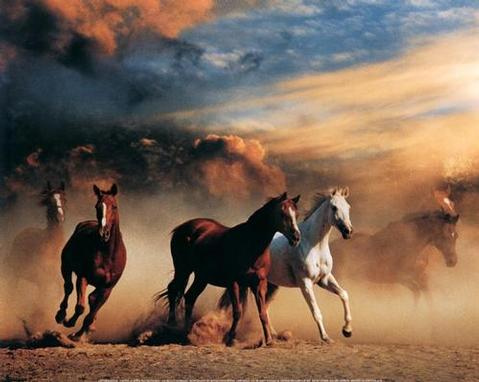
\includegraphics[width=10cm]{horses.png}
\end{figure}

\section{Project Management}

We have a very strong programming, mathematics, and data analysis background:

\begin{itemize}
	\item Dan Erickson: Sophomore in Computer Science Engineering, experience with numpy and MatLAB with image manipulation.
	\item Jessica Zhu: Junior in Computer Science Engineering, Minor image manipulation experience from EECS 280 assignment. 
	\item Ibrahim Alnassar: Sophomore in Computer Science Engineering, basic experience with Python, image manipulation, and image classification.
	\item Tim Sawyer: Sophomor in Industrial and Operations Engineering, basic Python and MatLAB experience.
	\item Josh Richman: Sophomore in Data Science Engineering, basic Python and image manipulation experience.
\end{itemize}

We all have very busy lives and will have other final projects and exams due around the same time as this project. Therefore, we will aim to complete our poster a week early. We will likely not completely finish by then, but we will have the majority done so we can focus on exams.

Tasks:
\begin{enumerate}
	\item Analyze real world uses for wavelet compressions.
	\item Write out section explaining the math of wavelet compressions and how it connects with the class.
	\item Write Python code to carry out wavelet compressions and perform wavelet compressions of black and white images.
	\item Analyze the compressed images and the implications and uses.
	\item Put together the poster.
\end{enumerate}

We will divide work into a group focused on tasks 1 and 2 and a group focused on tasks 3 and 4. Everyone will work together on the poster. The group focusing on tasks 1 and 2 will consist of Jessica, Ibrahim, and Tim. The other group will consist of Dan and Josh.

\end{document}
